\begin{flushleft}
	{\color{blue!50!green}\fbox{\fontfamily{qag}\bfseries\selectfont PHẦN I. Câu trắc nghiệm nhiều phương án lựa chọn}}
	\textit{\small (Thí sinh trả lời từ câu 1 đến câu 12. Mỗi câu hỏi thí sinh chỉ chọn một phương án.)}
\end{flushleft}
\setcounter{ex}{0}
\setcounter{bt}{0}

% Câu 1
\begin{ex}
	Cho hàm số $y = f(x)$ có bảng biến thiên như sau:
	\begin{center}
	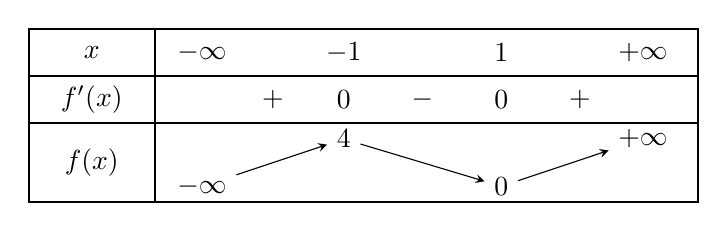
\begin{tikzpicture}[>=stealth,scale=1]
	  \draw[thick] (0,0) rectangle (8.5,-2.2);
	  \draw[thick] (0,-0.6) -- (8.5,-0.6);
	  \draw[thick] (0,-1.2) -- (8.5,-1.2);
	  \draw[thick] (1.6,0) -- (1.6,-2.2);
	  \node at (0.8,-0.3) {$x$};
	  \node at (0.8,-0.9) {$f'(x)$};
	  \node at (0.8,-1.7) {$f(x)$};
	  \node at (2.2,-0.3) {$-\infty$};
	  \node at (4.0,-0.3) {$-1$};
	  \node at (6.0,-0.3) {$1$};
	  \node at (7.8,-0.3) {$+\infty$};
	  \node at (3.1,-0.9) {$+$};
	  \node at (4.0,-0.9) {$0$};
	  \node at (5.0,-0.9) {$-$};
	  \node at (6.0,-0.9) {$0$};
	  \node at (7.0,-0.9) {$+$};
	  \node (p1) at (2.2,-2.0) {$-\infty$};
	  \node (p2) at (4.0,-1.4) {$4$};
	  \node (p3) at (6.0,-2.0) {$0$};
	  \node (p4) at (7.8,-1.4) {$+\infty$};
	  \draw[->] (p1) -- (p2);
	  \draw[->] (p2) -- (p3);
	  \draw[->] (p3) -- (p4);
	\end{tikzpicture}
	\end{center}
	Giá trị cực đại của hàm số là
	\choice
	{$-1$}
	{$1$}
	{\True $4$}
	{$0$}
	\loigiai{
		Theo bảng biến thiên, tại điểm $x = -1$ hàm số đạt cực đại và giá trị cực đại tương ứng là $y_{\text{CĐ}} = 4$.
	}
\end{ex}

% Câu 2
\begin{ex}
	Cho hàm số $y = f(x)$ có bảng biến thiên như sau:
	\begin{center}
	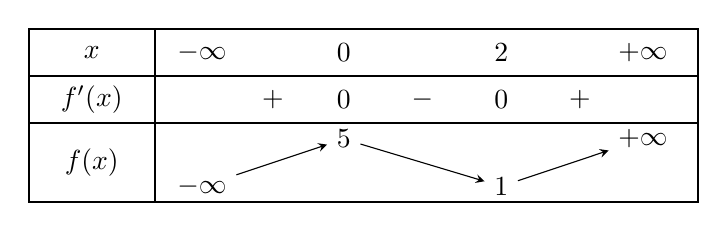
\begin{tikzpicture}[>=stealth,scale=1]
	  \draw[thick] (0,0) rectangle (8.5,-2.2);
	  \draw[thick] (0,-0.6) -- (8.5,-0.6);
	  \draw[thick] (0,-1.2) -- (8.5,-1.2);
	  \draw[thick] (1.6,0) -- (1.6,-2.2);
	  \node at (0.8,-0.3) {$x$};
	  \node at (0.8,-0.9) {$f'(x)$};
	  \node at (0.8,-1.7) {$f(x)$};
	  \node at (2.2,-0.3) {$-\infty$};
	  \node at (4.0,-0.3) {$0$};
	  \node at (6.0,-0.3) {$2$};
	  \node at (7.8,-0.3) {$+\infty$};
	  \node at (3.1,-0.9) {$+$};
	  \node at (4.0,-0.9) {$0$};
	  \node at (5.0,-0.9) {$-$};
	  \node at (6.0,-0.9) {$0$};
	  \node at (7.0,-0.9) {$+$};
	  \node (p1) at (2.2,-2.0) {$-\infty$};
	  \node (p2) at (4.0,-1.4) {$5$};
	  \node (p3) at (6.0,-2.0) {$1$};
	  \node (p4) at (7.8,-1.4) {$+\infty$};
	  \draw[->] (p1) -- (p2);
	  \draw[->] (p2) -- (p3);
	  \draw[->] (p3) -- (p4);
	\end{tikzpicture}
	\end{center}
	Điểm cực tiểu của hàm số đã cho là
	\choice
	{$x = 0$}
	{$x = 1$}
	{\True $x = 2$}
	{$x = 3$}
	\loigiai{
		Đạo hàm đổi dấu từ âm sang dương khi đi qua $x = 2$, do đó điểm cực tiểu của hàm số đã cho là $x = 2$.
	}
\end{ex}

% Câu 3
\begin{ex}
	\immini{
		Cho hàm số phân thức $y = \dfrac{ax^2 + bx + c}{px + q}$ ($a \ne 0, p \ne 0$, đa thức tử không chia hết cho đa thức mẫu) có đồ thị như hình bên. Đường tiệm cận xiên của đồ thị hàm số đã cho có phương trình là
		\choice
		{$y = x - 1$}
		{$y = -x + 1$}
		{\True $y = x + 1$}
		{$y = 2$}
	}{
		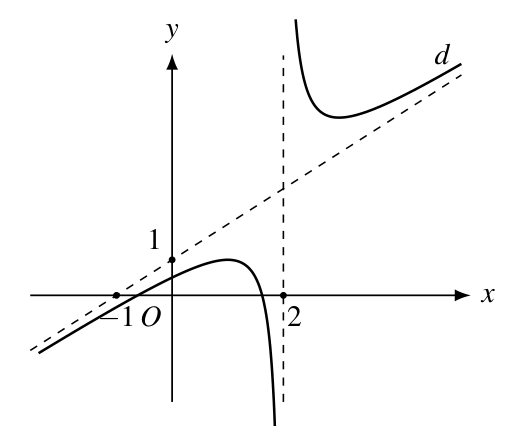
\includegraphics[width=4.6cm]{c3_hinh.png}
	}
	\loigiai{
		Đường tiệm cận xiên $d$ đi qua hai điểm $(-1; 0)$ và $(0; 1)$. Phương trình đường thẳng đi qua hai điểm này là:
		\[
		\dfrac{x}{-1} + \dfrac{y}{1} = 1 \iff y = x + 1.
		\]
	}
\end{ex}

% Câu 4
\begin{ex}
	\immini{
		Cho hàm số $y = \dfrac{ax + b}{cx + d}$ ($ac \ne 0, ad - bc \ne 0$) có đồ thị như hình bên. Đường tiệm cận đứng của đồ thị hàm số đã cho có phương trình là
		\choice
		{$y = -1$}
		{$y = 1$}
		{$x = 1$}
		{\True $x = -1$}
	}{
		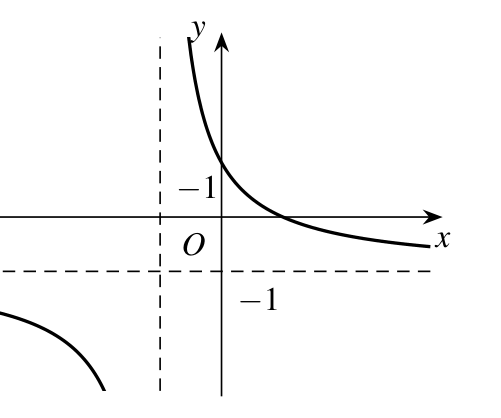
\includegraphics[width=4.5cm]{c4_hinh.png}
	}
	\loigiai{
		Đồ thị có đường tiệm cận đứng song song với trục $Oy$ và đi qua điểm $(-1; 0)$, suy ra phương trình đường tiệm cận đứng là $x = -1$.
	}
\end{ex}

% Câu 5
\begin{ex}
	\immini{
		Cho hàm số bậc ba $y = f(x)$ có đồ thị như hình bên. Tâm đối xứng của đồ thị là
		\choice
		{$I(0; 1)$}
		{\True $I(1; 1)$}
		{$I(1; 0)$}
		{$I(2; -1)$}
	}{
		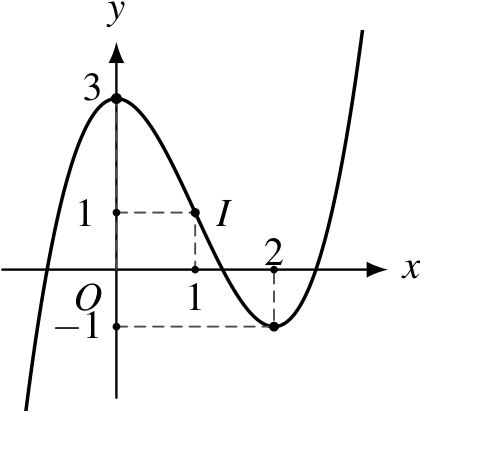
\includegraphics[width=4.5cm]{c5_hinh.png}
	}
	\loigiai{
		Tâm đối xứng của đồ thị hàm số bậc ba là điểm uốn $I$ nằm chính giữa điểm cực đại $(0; 3)$ và điểm cực tiểu $(2; -1)$.\\
		Tọa độ tâm đối xứng là $I\left(\dfrac{0 + 2}{2}; \dfrac{3 + (-1)}{2}\right) = I(1; 1)$.
	}
\end{ex}

% Câu 6
\begin{ex}
	\immini{
		Cho hàm số $y = \dfrac{ax + b}{cx + d}$ ($ac \ne 0, ad - bc \ne 0$) có đồ thị như hình bên. Hàm số nào dưới đây có đồ thị như hình vẽ?
		\choice
		{$y = \dfrac{x + 1}{x + 2}$}
		{$y = \dfrac{x - 5}{x - 2}$}
		{\True $y = \dfrac{x + 1}{x - 2}$}
		{$y = \dfrac{-x + 1}{x - 2}$}
	}{
		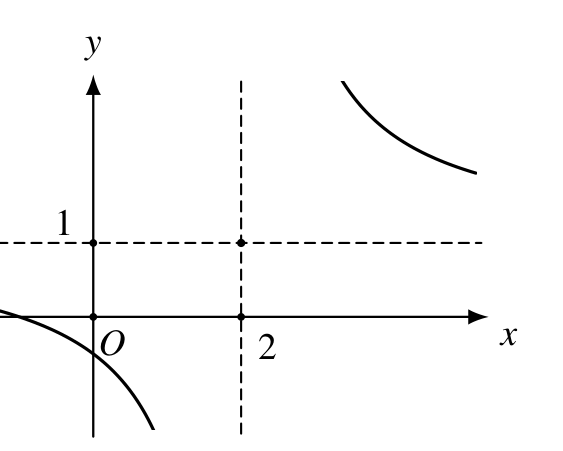
\includegraphics[width=4.8cm]{c6_hinh.png}
	}
	\loigiai{
		- Đồ thị có tiệm cận đứng $x = 2$, tiệm cận ngang $y = 1$.\\
		- Đồ thị cắt trục tung tại $\left(0; -\dfrac{1}{2}\right)$, cắt trục hoành tại $(-1; 0)$.\\
		Xét hàm số $y = \dfrac{x + 1}{x - 2}$, ta thấy thỏa mãn tất cả các điều kiện trên.
	}
\end{ex}

% Câu 7
\begin{ex}
	\immini{
		Cho hàm số bậc ba $y = f(x)$ có đồ thị như hình bên. Số điểm cực trị của hàm số là
		\choice
		{$0$}
		{$1$}
		{\True $2$}
		{$3$}
	}{
		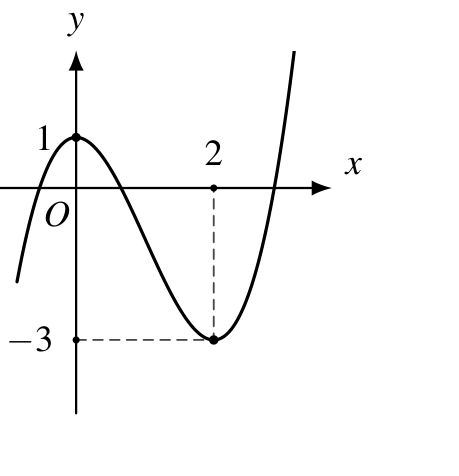
\includegraphics[width=4.4cm]{c7_hinh.png}
	}
	\loigiai{
		Quan sát đồ thị ta thấy đồ thị có một điểm cực đại và một điểm cực tiểu. Do đó hàm số có $2$ điểm cực trị.
	}
\end{ex}

% Câu 8
\begin{ex}
	Cho hàm số $y = f(x)$ có bảng biến thiên như sau:
	\begin{center}
	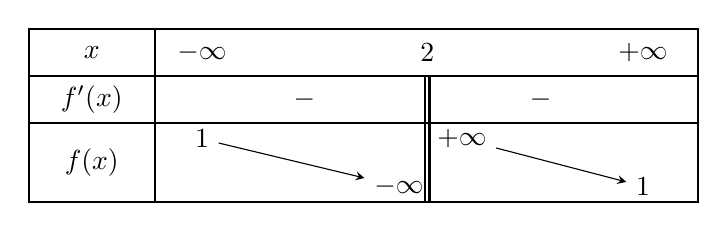
\begin{tikzpicture}[>=stealth,scale=1]
	  \draw[thick] (0,0) rectangle (8.5,-2.2);
	  \draw[thick] (0,-0.6) -- (8.5,-0.6);
	  \draw[thick] (0,-1.2) -- (8.5,-1.2);
	  \draw[thick] (1.6,0) -- (1.6,-2.2);
	  \draw[thick] (5.03,-0.6) -- (5.03,-2.2);
	  \draw[thick] (5.09,-0.6) -- (5.09,-2.2);
	  \node at (0.8,-0.3) {$x$};
	  \node at (0.8,-0.9) {$f'(x)$};
	  \node at (0.8,-1.7) {$f(x)$};
	  \node at (2.2,-0.3) {$-\infty$};
	  \node at (5.06,-0.3) {$2$};
	  \node at (7.8,-0.3) {$+\infty$};
	  \node at (3.5,-0.9) {$-$};
	  \node at (6.5,-0.9) {$-$};
	  \node (p1) at (2.2,-1.4) {$1$};
	  \node (p2) at (4.7,-2.0) {$-\infty$};
	  \node (p3) at (5.5,-1.4) {$+\infty$};
	  \node (p4) at (7.8,-2.0) {$1$};
	  \draw[->] (p1) -- (p2);
	  \draw[->] (p3) -- (p4);
	\end{tikzpicture}
	\end{center}
	Khẳng định nào sau đây đúng?
	\choice
	{Hàm số đồng biến trên khoảng $(-\infty; 2)$}
	{\True Hàm số nghịch biến trên từng khoảng $(-\infty; 2)$ và $(2; +\infty)$}
	{Hàm số đồng biến trên khoảng $(2; +\infty)$}
	{Hàm số nghịch biến trên $(-\infty; +\infty)$}
	\loigiai{
		Ta thấy đạo hàm mang dấu âm trên $(-\infty; 2)$ và $(2; +\infty)$, do đó hàm số nghịch biến trên từng khoảng $(-\infty; 2)$ và $(2; +\infty)$.
	}
\end{ex}

% Câu 9
\begin{ex}
	Cho hàm số $y = f(x)$ có bảng biến thiên như sau:
	\begin{center}
	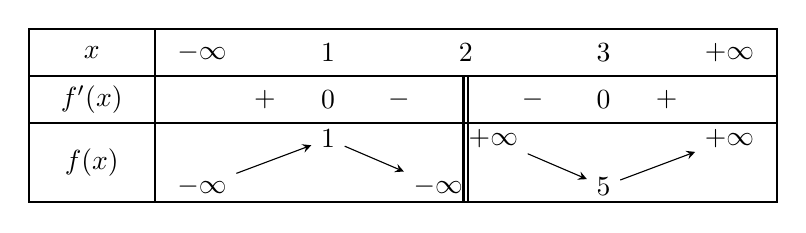
\begin{tikzpicture}[>=stealth,scale=1]
	  \draw[thick] (0,0) rectangle (9.5,-2.2);
	  \draw[thick] (0,-0.6) -- (9.5,-0.6);
	  \draw[thick] (0,-1.2) -- (9.5,-1.2);
	  \draw[thick] (1.6,0) -- (1.6,-2.2);
	  \draw[thick] (5.52,-0.6) -- (5.52,-2.2);
	  \draw[thick] (5.58,-0.6) -- (5.58,-2.2);
	  \node at (0.8,-0.3) {$x$};
	  \node at (0.8,-0.9) {$f'(x)$};
	  \node at (0.8,-1.7) {$f(x)$};
	  \node at (2.2,-0.3) {$-\infty$};
	  \node at (3.8,-0.3) {$1$};
	  \node at (5.55,-0.3) {$2$};
	  \node at (7.3,-0.3) {$3$};
	  \node at (8.9,-0.3) {$+\infty$};
	  \node at (3.0,-0.9) {$+$};
	  \node at (3.8,-0.9) {$0$};
	  \node at (4.7,-0.9) {$-$};
	  \node at (6.4,-0.9) {$-$};
	  \node at (7.3,-0.9) {$0$};
	  \node at (8.1,-0.9) {$+$};
	  \node (p1) at (2.2,-2.0) {$-\infty$};
	  \node (p2) at (3.8,-1.4) {$1$};
	  \node (p3) at (5.2,-2.0) {$-\infty$};
	  \node (p4) at (5.9,-1.4) {$+\infty$};
	  \node (p5) at (7.3,-2.0) {$5$};
	  \node (p6) at (8.9,-1.4) {$+\infty$};
	  \draw[->] (p1) -- (p2);
	  \draw[->] (p2) -- (p3);
	  \draw[->] (p4) -- (p5);
	  \draw[->] (p5) -- (p6);
	\end{tikzpicture}
	\end{center}
	Khoảng nào sau đây là một khoảng nghịch biến của hàm số?
	\choice
	{$(-\infty; 1)$}
	{$(1; 3)$}
	{\True $(1; 2)$}
	{$(3; +\infty)$}
	\loigiai{
		Dựa vào bảng biến thiên, đạo hàm âm trên các khoảng $(1; 2)$ và $(2; 3)$. Do đó $(1; 2)$ là một khoảng nghịch biến của hàm số.
	}
\end{ex}

% Câu 10
\begin{ex}
	\immini{
		Cho hàm số bậc ba $y = f(x)$ có đồ thị như hình bên. Điểm cực tiểu của hàm số đã cho là
		\choice
		{$x = -1$}
		{$x = 0$}
		{\True $x = 1$}
		{$x = 2$}
	}{
		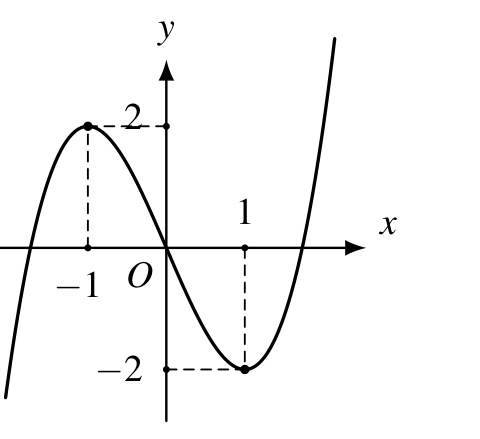
\includegraphics[width=4.4cm]{c10_hinh.png}
	}
	\loigiai{
		Điểm thấp nhất cục bộ của đồ thị là $(1; -1)$, do đó điểm cực tiểu của hàm số là $x = 1$.
	}
\end{ex}

% Câu 11
\begin{ex}
	\immini{
		Cho hàm số $y = \dfrac{ax + b}{cx + d}$ ($ac \ne 0, ad - bc \ne 0$) có đồ thị như hình bên. Tâm đối xứng của đồ thị là
		\choice
		{$I(1; 2)$}
		{$I(2; 1)$}
		{\True $I(-1; 2)$}
		{$I(2; -1)$}
	}{
		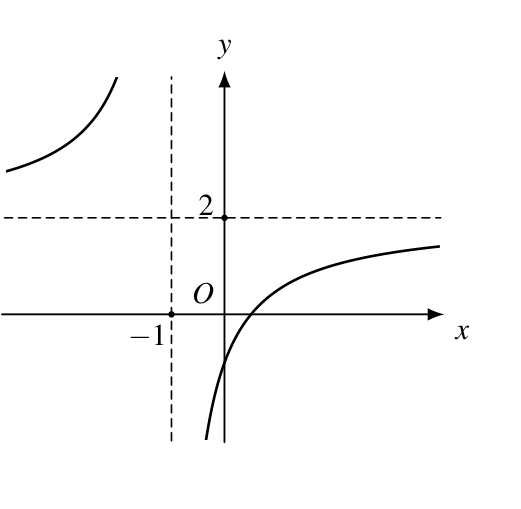
\includegraphics[width=4.6cm]{c11_hinh.png}
	}
	\loigiai{
		Đồ thị có tiệm cận đứng $x = -1$ và tiệm cận ngang $y = 2$. Tâm đối xứng của đồ thị là giao điểm của hai tiệm cận: $I(-1; 2)$.
	}
\end{ex}

% Câu 12
\begin{ex}
	\immini{
		Cho hàm số phân thức $y = \dfrac{ax^2 + bx + c}{px + q}$ ($a \ne 0, p \ne 0$, đa thức tử không chia hết cho đa thức mẫu) có đồ thị như hình bên. Đường tiệm cận xiên $d$ của đồ thị có phương trình là
		\choice
		{$y = x + 1$}
		{\True $y = x - 1$}
		{$y = -x - 1$}
		{$y = -1$}
	}{
		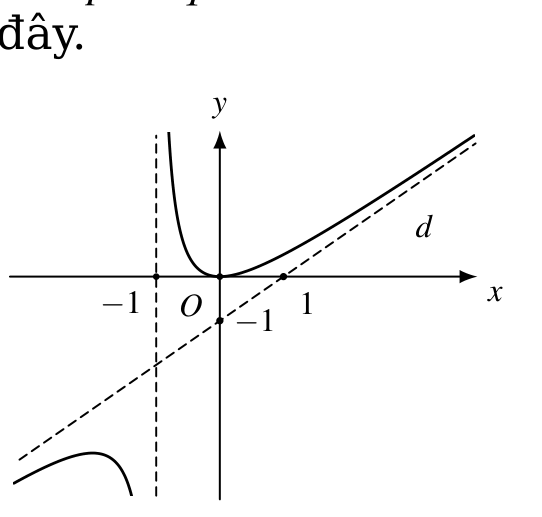
\includegraphics[width=4.8cm]{c12_hinh.png}
	}
	\loigiai{
		Đường thẳng $d$ đi qua các điểm $(1; 0)$ và $(0; -1)$, suy ra phương trình đường thẳng $d$ là $y = x - 1$.
	}
\end{ex}

\vspace{0.2cm}
\begin{flushleft}
	{\color{blue!50!green}\fbox{\fontfamily{qag}\bfseries\selectfont PHẦN II. Câu trắc nghiệm đúng sai}}
	\textit{\small (Thí sinh trả lời từ câu 1 đến câu 4. Trong mỗi ý a), b), c), d) ở mỗi câu, thí sinh chọn đúng hoặc sai.)}
\end{flushleft}
\setcounter{ex}{0}
\setcounter{bt}{0}

% Phần II Câu 1
\begin{ex}
	\immini{
		Cho hàm số bậc ba $y = f(x)$ có đồ thị như hình bên, trong đó điểm $I(0; 2)$ được đánh dấu. Xét tính đúng, sai của các phát biểu sau:
	}{
		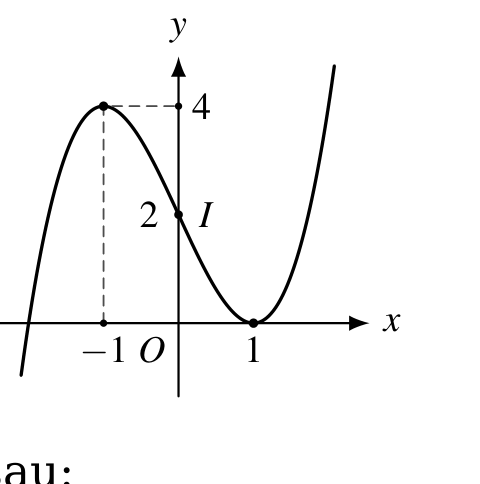
\includegraphics[width=4.6cm]{p2_c1_hinh.png}
	}
	\choiceTF
	{Hàm số đồng biến trên khoảng $(-1; 1)$}
	{\True Hàm số đạt cực đại tại điểm $x = -1$}
	{\True Giá trị cực tiểu của hàm số bằng $0$}
	{\True Điểm $I(0; 2)$ là tâm đối xứng của đồ thị}
	\loigiai{
		- Ý a) Sai: Trên khoảng $(-1; 1)$, đồ thị đi xuống từ trái sang phải nên hàm số nghịch biến.\\
		- Ý b) Đúng: Tại $x = -1$, đồ thị có điểm cực đại $(-1; 4)$, do đó hàm số đạt cực đại tại $x = -1$.\\
		- Ý c) Đúng: Điểm cực tiểu là $(1; 0)$, giá trị cực tiểu $y_{\text{CT}} = 0$.\\
		- Ý d) Đúng: Điểm uốn $I(0; 2)$ là trung điểm của đoạn nối hai điểm cực trị $(-1; 4)$ và $(1; 0)$, do đó $I(0; 2)$ là tâm đối xứng của đồ thị.
	}
\end{ex}

% Phần II Câu 2
\begin{ex}
	Cho các biểu diễn như dưới đây. Trong đó, Hình 1 và bảng biến thiên lần lượt là đồ thị và bảng biến thiên của hàm số $y = \dfrac{ax + b}{cx + d}$ ($ac \ne 0, ad - bc \ne 0$); Hình 2 là đồ thị của hàm số $y = \dfrac{mx^2 + nx + p}{qx + r}$ ($mq \ne 0$, đa thức tử không chia hết cho đa thức mẫu).
	\begin{center}
		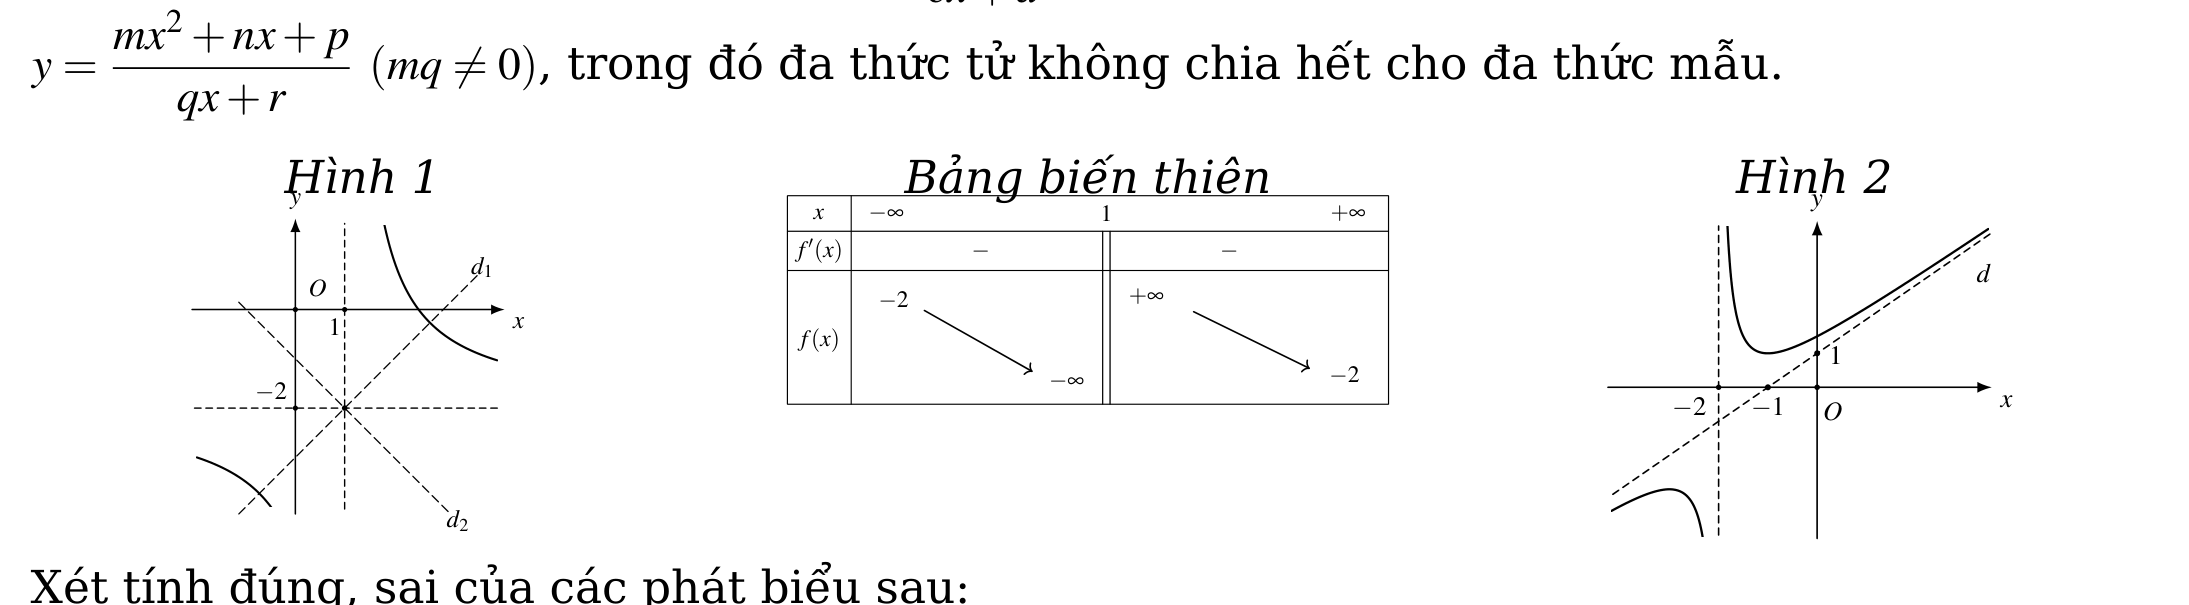
\includegraphics[width=14.0cm]{p2_c2_hinh_all.png}
	\end{center}
	Xét tính đúng, sai của các phát biểu sau:
	\choiceTF
	{\True Ở Hình 1, đường tiệm cận đứng của đồ thị là $x = 1$}
	{\True Ở Hình 1, cả $d_1$ và $d_2$ đều là trục đối xứng của đồ thị}
	{\True Bảng biến thiên cho thấy hàm số nghịch biến trên từng khoảng $(-\infty; 1)$ và $(1; +\infty)$}
	{Ở Hình 2, đường tiệm cận xiên $d$ có phương trình $y = x - 1$}
	\loigiai{
		- Ý a) Đúng: Đường tiệm cận đứng vuông góc với $Ox$ tại $x = 1$.\\
		- Ý b) Đúng: Đồ thị hàm phân thức bậc nhất trên bậc nhất có hai trục đối xứng là hai đường phân giác của các góc tạo bởi hai đường tiệm cận ($d_1$ và $d_2$).\\
		- Ý c) Đúng: Bảng biến thiên có dấu $f'(x) < 0$ trên $(-\infty; 1)$ và $(1; +\infty)$.\\
		- Ý d) Sai: Ở Hình 2, đường tiệm cận xiên $d$ đi qua $(-1; 0)$ và $(0; 1)$, có phương trình $y = x + 1$, không phải $y = x - 1$.
	}
\end{ex}

% Phần II Câu 3
\begin{ex}
	Cho hàm số $y = f(x) = x^3 - 3x + 1$ có đạo hàm $f'(x) = 3(x + 1)(x - 1)$ với mọi $x \in \mathbb{R}$. Xét tính đúng, sai của các phát biểu sau:
	\choiceTF
	{\True Tập xác định của hàm số là $\mathbb{R}$}
	{\True Hàm số đồng biến trên từng khoảng $(-\infty; -1)$ và $(1; +\infty)$}
	{Hàm số đạt cực tiểu tại $x = -1$}
	{\True Giá trị cực tiểu của hàm số bằng $-1$}
	\loigiai{
		- Ý a) Đúng: Hàm đa thức xác định trên $\mathbb{R}$.\\
		- Ý b) Đúng: $f'(x) > 0$ khi $x \in (-\infty; -1) \cup (1; +\infty)$.\\
		- Ý c) Sai: Đạo hàm đổi dấu từ dương sang âm qua $x = -1$, nên $x = -1$ là điểm cực đại.\\
		- Ý d) Đúng: Điểm cực tiểu là $x = 1$, giá trị cực tiểu $f(1) = 1 - 3 + 1 = -1$.
	}
\end{ex}

% Phần II Câu 4
\begin{ex}
	Cho hàm số $y = \dfrac{x^2}{x - 1}$. Xét tính đúng, sai của các phát biểu sau:
	\choiceTF
	{\True Tập xác định của hàm số là $\mathbb{R} \setminus \{1\}$}
	{\True Hàm số nghịch biến trên từng khoảng $(0; 1)$ và $(1; 2)$}
	{Hàm số đạt cực tiểu tại $x = 0$}
	{\True Đồ thị hàm số có đường tiệm cận xiên $y = x + 1$}
	\loigiai{
		Ta có $y = x + 1 + \dfrac{1}{x - 1}$ và $y' = \dfrac{x^2 - 2x}{(x - 1)^2} = \dfrac{x(x - 2)}{(x - 1)^2}$.\\
		- Ý a) Đúng: Mẫu số khác $0 \iff x \ne 1$.\\
		- Ý b) Đúng: $y' < 0$ khi $x \in (0; 1) \cup (1; 2)$.\\
		- Ý c) Sai: Đạo hàm đổi từ dương sang âm tại $x = 0$ nên $x = 0$ là điểm cực đại.\\
		- Ý d) Đúng: $\lim_{x \to \pm\infty} [y - (x + 1)] = \lim_{x \to \pm\infty} \dfrac{1}{x - 1} = 0$, nên tiệm cận xiên là $y = x + 1$.
	}
\end{ex}

\vspace{0.2cm}
\begin{flushleft}
	{\color{blue!50!green}\fbox{\fontfamily{qag}\bfseries\selectfont PHẦN III. Câu trắc nghiệm yêu cầu trả lời ngắn}}
	\textit{\small (Thí sinh trả lời từ câu 1 đến câu 6.)}
\end{flushleft}
\setcounter{ex}{0}
\setcounter{bt}{0}

% Phần III Câu 1
\begin{ex}
	Cho hàm số $y = f(x) = x^3 - 6x^2 + 9x + 1$ có đạo hàm $f'(x) = 3(x - 1)(x - 3)$ với mọi $x \in \mathbb{R}$. Tìm điểm cực đại của hàm số đã cho.
	\par\shortans[oly]{1}
	\loigiai{
		Ta có $f'(x) = 0 \iff x = 1$ hoặc $x = 3$. Đạo hàm đổi dấu từ dương sang âm khi qua $x = 1$, do đó hàm số đạt cực đại tại điểm $x = 1$.
	}
\end{ex}

% Phần III Câu 2
\begin{ex}
	Cho hàm số $y = g(x) = -x^3 + 3x + 2$ có đạo hàm $g'(x) = 3(1 - x^2)$ với mọi $x \in \mathbb{R}$. Giá trị cực đại của hàm số bằng bao nhiêu?
	\par\shortans[oly]{4}
	\loigiai{
		Ta có $g'(x) = 0 \iff x = \pm 1$. Hàm số đạt cực đại tại $x = 1$. Giá trị cực đại tương ứng là:
		\[
		g(1) = -(1)^3 + 3(1) + 2 = 4.
		\]
	}
\end{ex}

% Phần III Câu 3
\begin{ex}
	Cho hàm số $y = f(x) = \dfrac{2x + 1}{x - 1}$ có đạo hàm $f'(x) = -\dfrac{3}{(x - 1)^2}$ với mọi $x \ne 1$. Trong hai khoảng $(-\infty; 1)$ và $(1; +\infty)$, hàm số nghịch biến trên bao nhiêu khoảng?
	\par\shortans[oly]{2}
	\loigiai{
		Vì $f'(x) = -\dfrac{3}{(x - 1)^2} < 0$ với mọi $x \ne 1$, nên hàm số nghịch biến trên cả hai khoảng $(-\infty; 1)$ và $(1; +\infty)$. Do đó số khoảng nghịch biến là $2$.
	}
\end{ex}

% Phần III Câu 4
\begin{ex}
	Cho hàm số $y = f(x) = \dfrac{x^2}{x + 1}$ có đạo hàm $f'(x) = \dfrac{x(x + 2)}{(x + 1)^2}$ với mọi $x \ne -1$. Giá trị cực đại của hàm số bằng bao nhiêu?
	\par\shortans[oly]{-4}
	\loigiai{
		Phương trình $f'(x) = 0 \iff x = 0$ hoặc $x = -2$. Đạo hàm đổi dấu từ dương sang âm qua $x = -2$, do đó hàm số đạt cực đại tại $x = -2$ với giá trị cực đại là:
		\[
		f(-2) = \dfrac{(-2)^2}{-2 + 1} = \dfrac{4}{-1} = -4.
		\]
	}
\end{ex}

% Phần III Câu 5
\begin{ex}
	Cho hàm số $y = f(x) = x^3 - 3x^2 + 1$. Gọi $M$ và $m$ lần lượt là giá trị cực đại và giá trị cực tiểu của hàm số. Tính $M + m$.
	\par\shortans[oly]{-2}
	\loigiai{
		Ta có $f'(x) = 3x^2 - 6x = 3x(x - 2) = 0 \iff x = 0$ hoặc $x = 2$.\\
		- Tại $x = 0$: $M = f(0) = 1$ (giá trị cực đại).\\
		- Tại $x = 2$: $m = f(2) = 8 - 12 + 1 = -3$ (giá trị cực tiểu).\\
		Vậy $M + m = 1 + (-3) = -2$.
	}
\end{ex}

% Phần III Câu 6
\begin{ex}
	Cho hai hàm số $y = g(x) = \dfrac{2x + 1}{x - 1}$ và $y = h(x) = \dfrac{x^2 - x - 1}{x - 2}$. Gọi $a$ là tung độ tiệm cận ngang của đồ thị hàm số $g$, $b$ là hệ số tự do của tiệm cận xiên $y = x + b$ của đồ thị hàm số $h$. Tính $a + b$.
	\par\shortans[oly]{3}
	\loigiai{
		- Với hàm số $g(x) = \dfrac{2x + 1}{x - 1}$, tiệm cận ngang là $y = 2 \implies a = 2$.\\
		- Với hàm số $h(x) = \dfrac{x^2 - x - 1}{x - 2} = x + 1 + \dfrac{1}{x - 2}$, đường tiệm cận xiên là $y = x + 1 \implies b = 1$.\\
		Do đó $a + b = 2 + 1 = 3$.
	}
\end{ex}
